%!TEX root = ../main.tex

\graphicspath{{./figures/chapter2/}}


\chapter{Detection} \label{chap:chapter2}
\minitoc
\newpage


\section{Related work}


Hey, that's me: \cite{imbert_fishquant_2022}.

\subsection{Classical methods}

I have visited \ac{IGMM}.

\subsection{RS-FISH}

\subsection{DeepSpot}


\section{Automated spot detection}


\subsection{Spot detection}


\begin{figure}[h]
    \centering
    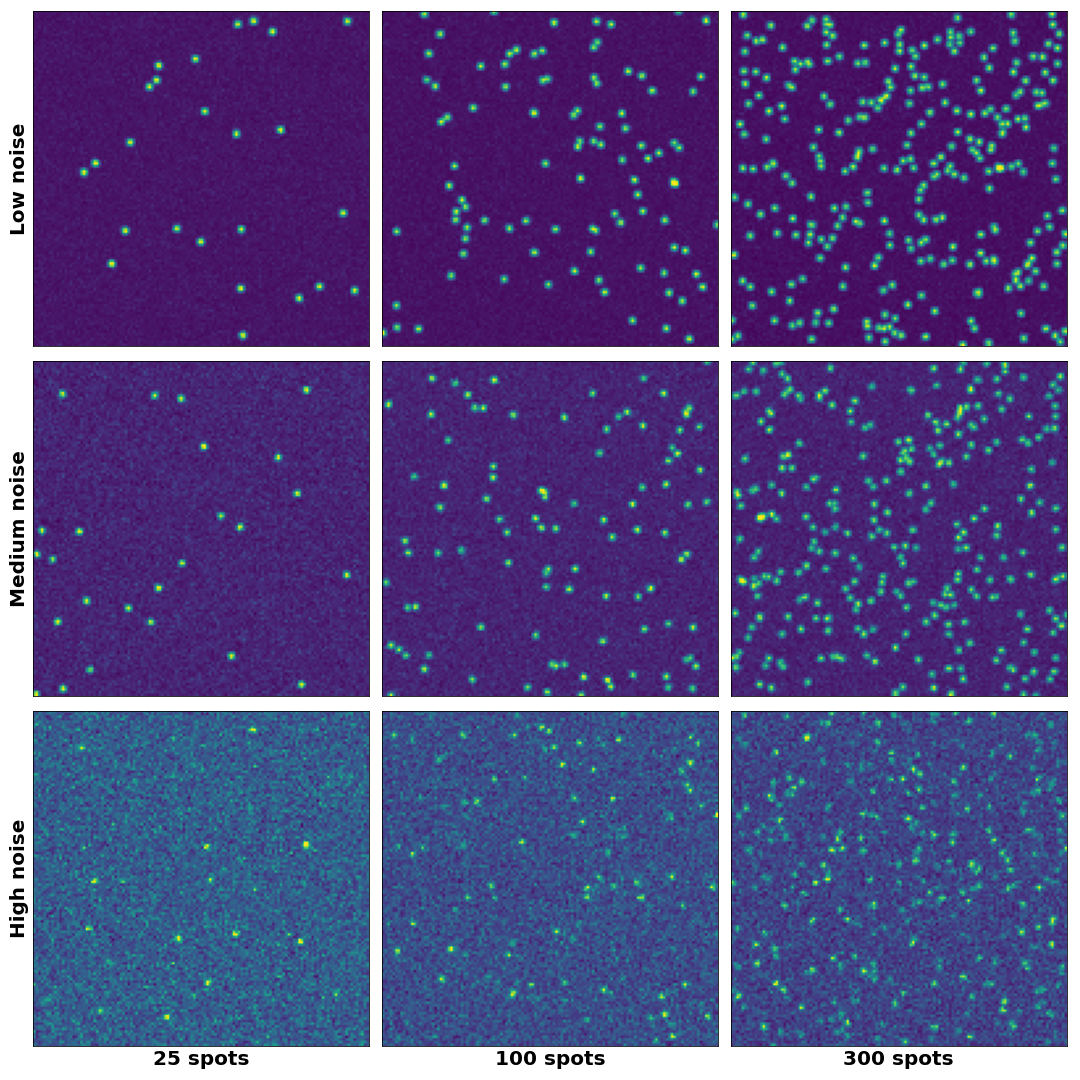
\includegraphics[width=0.75\textwidth]{figures/chapter2/spots_mosaic}
    \caption{A nice plot}
    \label{fig:testA}
\end{figure}


\subsection{Automated threshold}


\section{Dense region decomposition and cluster detection}


\subsection{Dense region detection}

\subsection{Dense region decomposition}

\subsection{Cluster detection}


\section{Additional features}


\subsection{Subpixel fitting}

\subsection{Spot colocalization}

% https://github.com/PreibischLab/RS-FISH/tree/master/documents/tool_comparison_for_paper